\section{Маршруты, цепи, циклы в графе. Метрические характеристики графа. Найти эксцентриситет 
вершины указанного графа, радиус, диаметр графа, центральные и периферийные вершины 
указанного графа.}

\begin{definition}
    \textit{Маршрут} (путь) в графе -- это конечная чередующаяся
    последовательность смежных вершин и ребер, соединяющих эти вершины.
\end{definition}

\textit{Маршрут} -- последовательность $v_1e_1v_2e_2 \dots e_{s-1}v_se_sv_{s+1} \dots v_k$,
в которой чередуются все вершины и ребра. $e_s=(v_s,v_{s+1})$.

\begin{definition}
    \textit{Длина маршрута} -- количество ребер в маршруте.
\end{definition}

\begin{definition}
    \textit{Нуль-маршрут} -- последовательность из одной вершины $v$.
\end{definition}

\begin{definition}
    \textit{Замкнутый маршрут (циклический)} -- последовательность, в которой
    совпадает начальная вершина с конечной. Иначе -- \textit{незамкнутый (открытый)}.
\end{definition}

\begin{definition}
    \textit{Цепь} -- незамкнутый маршрут, где все \textit{ребра} попарно различны.
\end{definition}

\begin{definition}
    \textit{Простая цепь} -- цепь, где все \textit{вершины} попарно различны.
\end{definition}

\begin{definition}
    \textit{Цикл} -- циклический маршрут, где все \textit{ребра} попарно различны.
\end{definition}

\begin{definition}
    \textit{Простой цикл} -- цикл, где все \textit{вершины, кроме первой и последней} попарно различны.
\end{definition}

\begin{theorem}
    Из любого цикла можно выделить простой цикл с той же начальной вершиной.
\end{theorem}

\begin{proof}
    Пусть $\exists \text{ цикл } v_1e_1v_2e_2 \dots v_se_s \dots v_je_j \dots v_ne_nv_1$.
    Если все вершины, кроме первой и последней, различны, то этот цикл простой. \\
    Допустим в цикле есть совпадающие вершины (не первая и не последняя) $v_s=v_j$. Тогда
    удаляем часть маршрута между этими вершинами.
    \begin{align*}
        v_1e_1v_2e_2 \dots v_se_s \dots v_je_j \dots v_ne_nv_1 \Rightarrow
        v_1e_1v_2e_2 \dots v_se_j \dots v_ne_nv_1
    \end{align*}
    Так как $v_s=v_j$, то полученная последовательность является маршрутом.
    Продолжая получим простой цикл.
\end{proof}

\begin{theorem}
    Из любой цепи можно выделить простую цепь с теми же
    начальными и конечными вершинами (док-во аналогично).
\end{theorem}

\begin{definition}
    \textit{Связанные вершины в графе} -- $\exists$ маршрут
    с началом в первой вершине и концом на второй.
\end{definition}

\begin{definition}
    \textit{Связный граф} -- две любые вершины являются \textit{связанными}.
\end{definition}

Пусть $G(V,E)$ -- связный неориентированный граф ($v_i,v_j \in V$).

\begin{definition}
    \textit{Расстояние между вершинами, $d(v_i,v_j)$} -- длина
    \textit{кратчайшего} маршрута между этими вершинами.
\end{definition}

\begin{definition}
    \textit{Эксцентриситет вершины графа} -- число, максимальное
    из расстояний между этой вершиной и всеми остальными вершинами.
    \begin{align*}
        \varepsilon(v_i) = \max d(v_i,v_j), v_j \in V, i \neq j
    \end{align*}
\end{definition}

\begin{definition}
    \textit{Диаметр графа, $D(G)$} -- максимальный из всех эксцентриситетов
    вершин данного графа.
\end{definition}

\begin{definition}
    \textit{Радиус графа, $R(G)$} -- минимальный из всех эксцентриситетов
    вершин данного графа.
\end{definition}

\begin{definition}
    \textit{Периферическая вершина} -- ее эксцентриситет равен диаметру.
\end{definition}

\begin{definition}
    \textit{Центральная вершина} -- ее эксцентриситет равен радиусу.
\end{definition}

\begin{definition}
    \textit{Центр графа} -- множество всех центральных вершин.
\end{definition}

Пример: Найти эксцентриситеты вершин, диаметр и радиус графа,
периферийные и центральные вершины.

\begin{figure}[h]
    \centering
    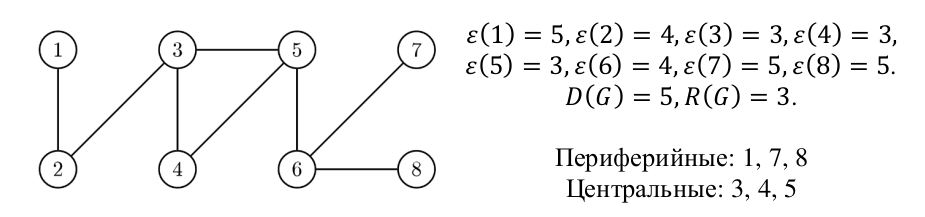
\includegraphics[width=\textwidth]{4.png}
\end{figure}